% This is LLNCS.DEM the demonstration file of
% the LaTeX macro package from Springer-Verlag
% for Lecture Notes in Computer Science,
% version 2.3 for LaTeX2e
%
\documentclass{llncs}
%
\usepackage{makeidx}  % allows for indexgeneration
\usepackage{graphicx}
\usepackage{amssymb}
\usepackage{listings}
\usepackage{tabularx}
\usepackage{booktabs}
\usepackage{subscript}
\lstset{breaklines=true, basicstyle=\scriptsize\ttfamily}

%
\begin{document}
%
\frontmatter          % for the preliminaries
%
\pagestyle{headings}  % switches on printing of running heads
%\addtocmark{Hamiltonian Mechanics} % additional mark in the TOC
%
%
\mainmatter              % start of the contributions
%
\title{Semantic Publishing - Research Life Cycle}

%
\titlerunning{Semantic Publishing - Research Life Cycle}  % abbreviated title (for running head)
%                                     also used for the TOC unless
%                                     \toctitle is used
%
\author{Aleix Garrido\inst{1} \and Jose Manuel Gomez-Perez\inst{1} \and Boris Villazon-Terrazas\inst{1}}
%
\authorrunning{Garrido et al.}   % abbreviated author list (for running head)
%
%%%% list of authors for the TOC (use if author list has to be modified)
%\tocauthor{Panos Alexopoulos, Manolis Wallace}
%
\institute{
iSOCO, Intelligent Software Components S.A., Av. del
Partenon, 16-18, 1-7, 28042, Madrid, Spain,\\
\email{\{agarrido,jmgomez,bvillazon\}@isoco.com}}


%\maketitle              % typeset the title of the contribution

%**************************************************************
%**************************************************************
%**************************************************************


\begin{abstract}


\end{abstract}

\section{Introduction}\label{sec:Introduction}
Research is intended for the betterment of society and the world, and science is incremental. Important discoveries and developments are built on top of previous research efforts, which are validated by peer scientists and accepted for publication in scholarly communications. However, the process of identifying experts in a particular field, which can be suitable reviewers for a particular article can be cumbersome and costly.

In this paper, we describe the system that aims to help journal editors, conference and workshop chairs on identifying suitable reviewers for a particular paper, by providing a nice visualization of related authors and papers. To this end, the system relies on an innovative social network visualization, namely Collaboration Sphere, CSs. 

In a nuthshell, the visual metaphor called Collaboration Spheres allow search through exploration of scientific social networks based on a combination of people and information objects. This search paradigm is built around the use of customizable contexts that act as intuitive examples conducted by the users. This tool eases collaboration, expert finding and access to relevant information.

It is worth mentioning that in this case we plug the Collaboration Spheres over the APA enriched dataset, but the CSs are customizable and they can plug to other datasets, coming from different domains, with minor configuration changes.




\section{Reuse of scientific work}\label{sec:RelatedWork}
Reuse of scientific work, including search and exploration of relevant scientific experiments in scientific social networks (Collaboration Spheres). Wf4Ever 


\section{Reviewer finder}\label{sec:Motivation}
%introducción
The Collaboration Spheres are illustrated by a web application that covers the process
of finding a good reviewer for a specific article or publication. The Collaboration Spheres are a visual metaphor of concentric circles where the most important part (the article) the level of importance decreases as we move away from the center. The metaphor is helped by the use of intuitive colors and iconography. In that way, the user experiences a level of trust based on closeness. The process is driven by actions performed by the user while creating different contexts near the article towards his/her final objective which is to find good reviewers. Each action allows the modification of the search parameters in an intuitive way and offers summaries of information that may help on understanding the available resources.\\
\subsection{Interface Description}
The user interface has been designed in order to keep a minimalist layout that
makes user experience smooth and simple. The screen is easily divided in four
different parts:
\begin{description}
\item[Spheres]The main part displays a set of concentric circles. These circles
have two different functionalities. On the one hand, the center of the circles
contains the main article for which we are looking for reviewers. Its adjacent
circle is the place where search queries are defined through dropping elements
from the lists of items(see Lists) for creating contexts. On the other hand the
two external circles offer the results of the reviewer finder. The results are
small icons that use different colors depending on the relative quality of the
recommendation (green for the best results, yellow for medium, and red for weak
recommendations). The icon may have a warning sign associated if a conflict of
interest (such as previous co-authors or same organization) is detected for the
recommended reviewer.
\item[Lists]A total of six lists are loaded on the right side of the screen.
They are divided in two columns: authors and articles. Each column has three
lists. The lists on the first column are: list of authors of the main article,
list of previous co-authors of the main authors and a list of authors which have
worked on related topics to the article to be reviewed. The lists on the second
column are: articles of the main authors, articles of previous co-authors and
topic related articles. By preselecting the listed item we ease the task for the user by removing non relevant information and keeping only elements oriented for the recommendation task. All the items of the lists are draggable and can be
dropped on the Spheres in order to customize the context.
\item[Tag Cloud]A tag cloud that gathers the most representative topics of the
contexts that are created by the user is placed beneath the Spheres. The tag
cloud allows the understanding of the search and results at a glance.
\item[Information box]Each element of the lists and the spheres is clickable. If
they are clicked, a box of information placed on the right-bottom corner of the
screen loads a brief summary of information, together with a link to its uri and
a list of relevant topics for the current context. The purpose of this box is to offer quick summaries of every element that the user wants to inspect without the need of leaving the Collaboration Spheres page.
\end{description}
\begin{figure}[!hbt]
\centering
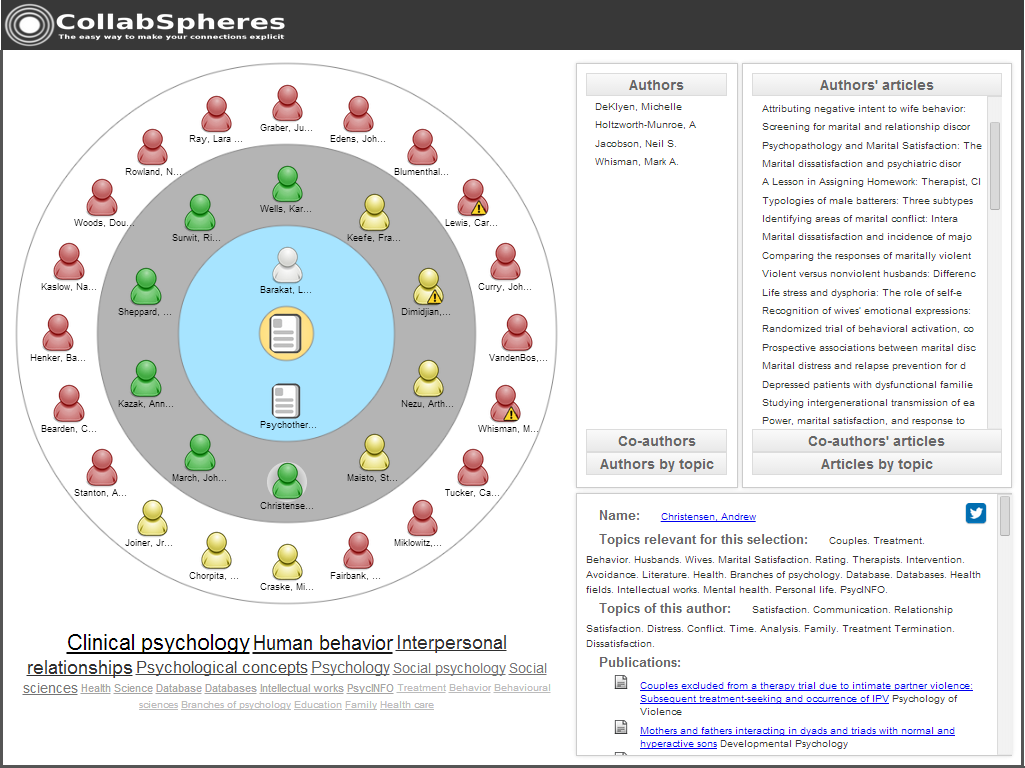
\includegraphics[scale=0.3]{img/CollabAPA.png}
\caption{User interface screenshot}
\label{fig:screenshot}
\end{figure}
\subsection{Basic Architecture}
The architecture of the system consists of three modules. Each module provides
the needed information to the others creating a complete system.
\begin{description}
\item[Data Module]The Collaboration Spheres use data provided by the APA VIVO\footnote{\url{https://vivo.apa.org/}} platform, which is an RDF dataset holding authors, publications and additional data from the psychology domain. The base dataset is imported to our repository, transformed and with topics from the titles and abstracts that have been extracted using the TextRazor\footnote{\url{http://www.textrazor.com/} TextRazor provides topic extraction and additional Wikipedia URIs for different categories.} API and KT (Knowledge Tagger) working together with a Thesaurus. The transformation and enrichment using topics for the authors and articles are made in order to get an explicit represenation that improves the querying process in terms of complexity and time. The Post-processing calculations are used to add a weight value for each topic in every article and to assess an expertise value to the authors. These assigned weights are the key part of the recommendation. The final dataset is stored in a Virtuoso Triplestore accessible via HTTP SPARQL queries.
\item[Web Services]The communications between the Data Module and the Front End are performed by the Web Services. It is a web project that triggers different SPARQL queries by using JENA under user request. The results are processed and returned via REST-JSON to the Front End.
\item[Front End]A web application with a browsable interface that is directly available for the users. The interface reacts to user actions and throws different Ajax queries to the REST Web Services. It has been developed in HTML5, using also javascript, jQuery and CSS. 
\end{description}
\begin{figure}[!hbt]
\centering
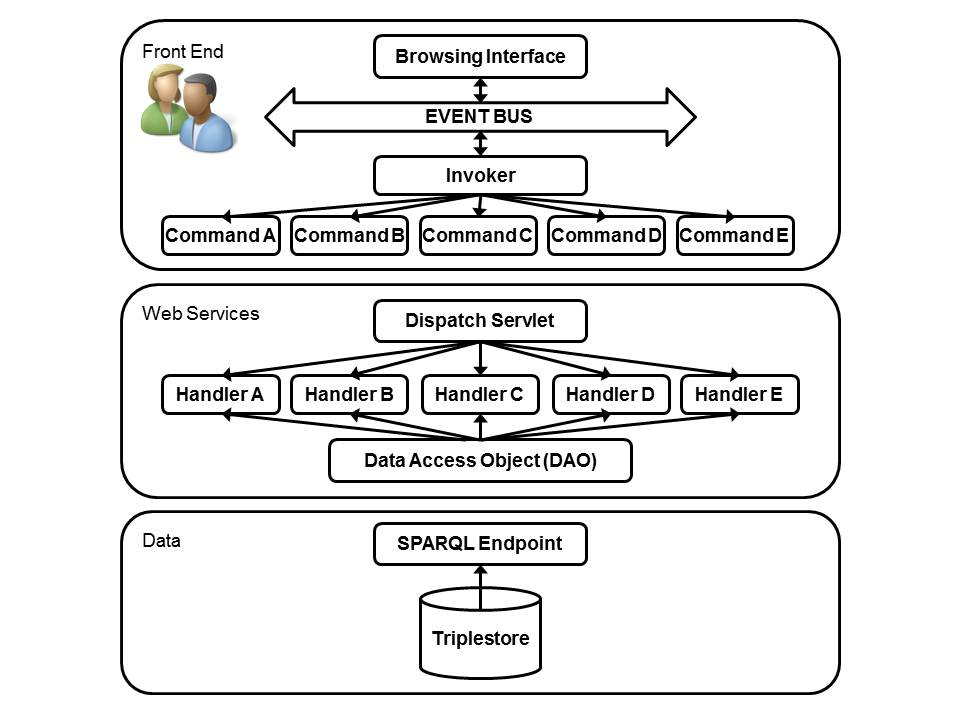
\includegraphics[scale=0.3]{img/APAarchitecture.jpg}
\caption{Basic architecture}
\label{fig:arch}
\end{figure}
\subsection{Scenario}
In this scenario the editor in chief of the Journal of Personality and Social
Psychology\footnote{\url{http://www.apa.org/pubs/journals/psp/}} is trying to
select reviewers for a submission they have just received. The first step will
be to open the collaboration spheres for that Article: 
\begin{itemize}
  \item The selected Article is called "Attachment change processes in the early
years of marriage" \footnote{\url{http://vivo.apa.org/individual/n61963}}.
  \item Then we can launch the Collaboration Spheres for the Article
\footnote{\url{http://apaproject.isoco.com/index.html?id=http://vivo.apa.org/individual/n61963}}.
\end{itemize}
As we can see, at the tag cloud shows the most relevant topics for the Article
placed in the center of the Collaboration Spheres and we get a preliminary set
of recommended reviewers for it.\\
Since we want to define a bit better the topics for our context, i.e. the
special issue, and, in order to get better recommendations, we will add an
article of our interest (can be found at the “Articles by Topic section), which
is very related to the topics of the special issue. We select the following
article in the “Articles by topic” panel on the right and drag and drop it into
the blue circle of the context of interest:
\begin{itemize}
  \item The added article is "Adult attachment and the transition to parenthood"
\footnote{\url{http://vivo.apa.org/individual/n5724}}.
\end{itemize}
Now the editor in chief will include some of the members of the Editorial Board
(Interpersonal Relations and Group Processes
Section\footnote{\url{http://www.apa.org/pubs/journals/psp/edboard-irgp.aspx}}),
who will serve as exemplars of the knowledge required to properly evaluate the
submissions which are received. Suitable reviewers will therefore be
knowledgeable of (part of) those topics. This way we increase the alignment
between the related topics in the expertise of our editors and the recommended
experts for reviewing the article. In this case, the editor in chief adds:
\begin{itemize}
  \item Consulting Editors:
  \begin{itemize}
    \item Bolger, Niall\footnote{\url{http://vivo.apa.org/individual/n41433}}
    \item Algoe, Sara B.\footnote{\url{http://vivo.apa.org/individual/n59044}}
  \end{itemize}
  \item Associate Editors:
  \begin{itemize}
      \item Finkel, Eli J.\footnote{\url{http://vivo.apa.org/individual/n36079}}
      \item Gable, Shelly L.\footnote{\url{http://vivo.apa.org/individual/n37385}}
  \end{itemize}
\end{itemize}
We can see at every addition how the main topics change in the tag cloud and how
the recommendations are adjusted to the context. When the editor in chief adds
the last of the associate editors, the relevance of the different related topics
seems to be uniformly distributed. The editor in chief then may want to
reconsider the composition of the board and replace some of the editors (e.g.
Gable with another expert with knowledge about other topics more, which the
editor in chief finds especially relevant for the special issue).  In this case,
the editor in chief selects an author who brings in expertise related to topics
like alcohol abuse:
\begin{itemize}
  \item Zywiak, William H.\footnote{\url{http://vivo.apa.org/individual/n8844}}
\end{itemize}
In addition to the summary that we provide for each author and article, the
system can also launch a Twitter search that covers his/her/its intersection
with the most relevant topics of the context of interest.



\section{Evaluation}\label{sec:Evaluation}
Validation and evaluation of the experiment results and materials (Completeness, Stability, Reliability). 



\section{Conclusions and Future Work}\label{sec:Conclusions}
This is the worst conclusions ever ...

In this paper we have described a system for finding reviewers for scholarly publications, developed in the context of a joint project with APA. Future work includes the evaluation of the tool in real case scenario with the participation of experts. 


%*****************************************************************************************************************



\section*{Acknowledgments}

This work was supported by SmartContent project.
%and PARLANCE (www.parlanceproject.eu, grant number 287615).



% ---- Bibliography ----
%

\bibliography{bibliography}
\bibliographystyle{plain}



\clearpage
\addtocmark[2]{Author Index} % additional numbered TOC entry
\renewcommand{\indexname}{Author Index}
\printindex \clearpage
\addtocmark[2]{Subject Index} % additional numbered TOC entry
\markboth{Subject Index}{Subject Index}
\renewcommand{\indexname}{Subject Index}
\input{subjidx.ind} 
\end{document}
